\documentclass[a4paper,10pt]{article}

\usepackage{color}
\usepackage{xcolor}
\usepackage{tikz}
\usepackage{amsmath}
\usepackage{amssymb}
\usepackage{amsthm}
\usepackage{graphicx}
\usepackage{mathtools}
\usepackage{wrapfig}
\usepackage{multirow}
\usepackage{comment}
\usepackage{natbib}
%\usepackage{float}
\usepackage{appendix}
\usepackage{subfig}
\usepackage{enumitem}
\usepackage{newfloat}
\usepackage[utf8]{inputenc}
\usepackage{floatrow}
\usepackage{bm}

\usetikzlibrary{calc}
\usetikzlibrary{fit}
\usetikzlibrary{decorations.shapes,shapes.misc,calc, positioning, hobby, backgrounds}

\tikzset{decorate sep/.style 2 args=
{decorate,decoration={shape backgrounds,shape=circle,shape size=#1,shape sep=#2}}}

%\DeclarePairedDelimiter{\floor}{\lfloor}{\rightfloor}
%\DeclarePairedDelimiter{\ceil}{\lceil}{\rceil}

\newcommand{\halflength}{\ensuremath{\floor{\frac{m}{2}}}}
\newcommand{\floor}[1]{\left \lfloor #1 \right \rfloor}
\newcommand{\ceil}[1]{\left \lceil #1 \right \rceil}

\newtheorem{theorem}{Theorem}[section]
\newtheorem{corollary}[theorem]{Corollary}
\newtheorem{lemma}[theorem]{Lemma}

\theoremstyle{definition}
\newtheorem{definition}[theorem]{Definition}

\theoremstyle{definition}
\newtheorem{example}[theorem]{Example}
 
\theoremstyle{remark}
\newtheorem*{remark}{Remark}

\theoremstyle{definition}
\newtheorem*{note}{Note}

\DeclareFloatingEnvironment[fileext=los,
    listname={List of Example Figures},
    name=Example Figure,
    placement=tbhp,
    within=section,]{examplefigure}

\DeclareFloatingEnvironment[fileext=los,
    listname={List of myFigures},
    name=Figure,
    placement=tbhp,
    within=section,]{myfigure}      

\title{A graph Patrol Problem with a random attacker on edges}
\date{\today}
\author{Thomas Lowbridge \\ School of Mathematical Sciences \\ University of Nottingham}

\bibliographystyle{plain}

\begin{document}

\pagestyle{empty}
{
  \renewcommand{\thispagestyle}[1]{}
  \maketitle
  \tableofcontents  
}
\clearpage
\pagestyle{plain}


\setlength{\parindent}{0pt}
\setlength{\parskip}{1em}

\newpage
\pagenumbering{arabic}
\section{Introduction to a random attacker patroller game with attacks on edges}
The model has a undirected graph $Q=(N,E)$ with a set of nodes labelled $1$ to $n$, $N=\{1,...,n \}$ and a set of edges linking the nodes which are a subset of $E_{comp}=\{(i,j) \, | \, i,j \in N \}$. The adjacency matrix $a=(a_{i,j})_{i,j \in N}$ has $a_{i,j}=1$ if $i$ and $j$ are adjacent and $a_{i,j}=0$ if they are not adjacent. By definition we will use $a_{i,1}=1 \quad \forall i \in N$.

\begin{note}
We note that we have no edge $(i,i)$ , but the node is still adjacent to its self. Also note that edge $(i,j)=(j,i)$ Hence we will assume that $i \leq j$ to uniquely describe and edge.
\end{note}

An attacker will arrive at some continuous position along an edge on the graph. The attackers arrive according to a Poisson process with rate $\Lambda$ and will choose to attack edge $(i,j)$ with probability $p_{i,j}$, hence by Poisson thinning we will arrive on the edge with a Poisson process with rate $\lambda_{i,j}=p_{i,j} \Lambda$. Once a node is picked the attacker will pick a position along the unit length line according to some distribution function $f_{i,j}(x)$ (with support $x \in [0,1]$ and c.d.f $F_{i,j}(x)$). The length of an attack is a random variable $X_{i,j}$, which measures the amount of time before completion.

The patroller, will use some walk (with possible waiting) to partol the graph. We assume that the walk along an edge is uniform in real time, and that the edges are of unit length. So after making the decision of which node to move to they will arrive one unit later, with linear (continuous) movement along the edge. With each completing attack costing, $c_{i,j}$

This means that once an edge is picked, it is `renewed' as normal, however their may be a residual amount of attacks left behind the patroller, while all currently commencing attacks that are not complete when the patroller reaches them are caught. Because an edge can be traversed $i$ to $j$ or $j$ to $i$, it will matter which way we just traversed as to where the residual amount of attacker may be left.

So we will formulate the state space as the delineation of separate edges. $\Omega=\{ (\bm{s},\bm{d}) \, | \, s_{i,j}=1,2,....  \quad d_{i,j}=0 \text{ or } 1 \, \forall i,j \in N \}$ , where $\bm{s}=(s_{i,j})_{(i,j) in E}$ has $s_{i,j}$ represent the number of time periods since we last decided to traverse the edge $(i,j)$ and $d_{i,j}=0$ if we traversed it from left to right, i.e we traversed $(i,j)$ otherwise if $d_{i,j}=1$ if we traversed it from right to left i.e we traversed $(j,i)$.

The $s_{i,j}$ increment by 1 unless the edge was just traversed, in which case it then resets to 1. The $d_{i,j}$ remain unchanged unless the edge was just traversed, in which case it becomes 0 if we traversed $i$ to $j$ and 1 if we traversed $j$ to $i$. The current node is found by analysing which of the $s_{i,j}=1$ and if $d_{i,j}=0$ (then we are at node $j$) or if $d_{j,i}=1$ (then we are node $i$). Let $l(\bm{s},\bm{d})$ represent the current node found by the rule above, i.e argument of the min and then decide which side by using direction.

As the future of the process is independent of its past, the process can be formulated as a Markov Decision Process(MDP), where at the end of the period the patroller chooses which adjacent node to visit (and thus cover an edge). Thus the action space is $\mathcal{A}=\{ j \, | \, a_{l(\bm{s},\bm{d}),j}=1 \}$, with a determinsitic stationary policy, $\pi : \Omega \rightarrow \mathcal{A}$.

The transitions are purely determinsitic, $(\bm{s},\bm{d})$ with the decision to move to node $i \in \mathcal{A}$ transitions the state to $(\widetilde{\bm{s}},\widetilde{\bm{d}})$. Where $\widetilde{s_{k,j}}=s_{k,j}+1$ if $k \neq i,j \neq i$ and $\widetilde{s_{k,j}}=1$ if $k=i \text{ or } j=i$. Also $\widetilde{d_{k,j}}=d_{k,j}$ if $k \neq i, j \neq i$ and $\widetilde{d_{k,j}}=0$ if $j=i$ and $\widetilde{d_{k,j}}=1$ if $k=i$.

To write down the cost function, which will be dependent on the state $(\bm{s},\bm{d})$ and the action to visit node $i$ is chosen, we will look at the expected cost incurred at all edges and sum these costs for the next time period.

The cost incurred in the next time period at edge $(k,j)$ is

\begin{align}
C_{k,j}(\bm{s},\bm{d},i)&= \begin{cases}
c_{k,j} \lambda_{k,j} \int_{0}^{1} f_{k,j}(y) \left(\int_{0}^{s_{k,j}} P(t-1 < X_{k,j} \leq t) dt \right) dy \text{ If same direction}\\
c_{k,j} \lambda_{k,j} \int_{0}^{1} f_{k,j}(y) \left(\int_{0}^{s_{k,j}+1-2y} P(t-1 < X_{k,j} \leq t) dt \right) dy \text{ If opposite direction}
\end{cases} \nonumber \\
&= \begin{cases}
c_{k,j} \lambda_{k,j} E_{Y} \left[\int_{0}^{s_{k,j}} P(t-1 < X_{k,j} \leq t) dt \right] \text{ If same direction}\\
c_{k,j} \lambda_{k,j} E_{Y} \left[\int_{0}^{s_{k,j}+1-2Y} P(t-1 < X_{k,j} \leq t) dt \right] \text{ If opposite direction}
\end{cases} \nonumber \\
&= \begin{cases}
c_{k,j} \lambda_{k,j} \int_{0}^{s_{k,j}} P(t-1 < X_{k,j} \leq t) dt \text{ If same direction}\\
c_{k,j} \lambda_{k,j} E_{Y} \left[\int_{0}^{s_{k,j}+1-2Y} P(t-1 < X_{k,j} \leq t) dt \right] \text{ If opposite direction}
\end{cases} \nonumber \\
&= \begin{cases}
c_{k,j} \lambda_{k,j} \int_{s_{k,j}-1}^{s_{k,j}} P(X_{k,j} \leq t) dt \text{ If same direction}\\
c_{k,j} \lambda_{k,j} E_{Y} \left[\int_{s_{k,j}-2Y}^{s_{k,j}+1-2Y} P(X_{k,j} \leq t) dt \right] \text{ If opposite direction}
\end{cases}
\end{align}


\begin{note}
We note that the cost depends on whether we are going to traverse the edge in the same direction as last time or not. The conditions formally are
\begin{itemize}
\item Same direction:
$ l(\bm{s},\bm{d}) \leq i  \text{ and } d_{l(\bm{s},\bm{d}),i}=0$
or
$ l(\bm{s},\bm{d}) > i \text{ and } d_{l(\bm{s},\bm{d}),i}=1$
\item Opposite direction:
$ l(\bm{s},\bm{d}) \leq i  \text{ and } d_{l(\bm{s},\bm{d}),i}=1$
or
$ l(\bm{s},\bm{d}) > i  \text{ and } d_{l(\bm{s},\bm{d}),i}=0$
\end{itemize}
\end{note}
 
With the total cost incurred being $C(\bm{s},\bm{d},i)=\sum\limits_{(k,j) \in E} C_{k,j}(\bm{s},\bm{d},i)$

We will now assume that the attack time is bounded, i.e $X_{k,j} \leq B_{k,j}$, where $B_{k,j}=\min \{ b \, | b \in \mathbb{Z}^{+} , P(X_{k,j} \leq b)=1 \}$. Now are cost functions are going to be the same for $s_{k,j} \geq B_{k,j}+1$ we can restrict our state space to having $s_{k,j} \leq B_{k,j}+1$, so $\Omega= \{(\bm{s},\bm{d}) \, | \, s_{k,j}=1,2,...,B_{k,j} \, d_{k,j}=0 \text{ or } 1 \, \forall (k,j) \in E \}$ we a slightly modified transition that $\widetilde{s_{k,j}}=\min \{s_{k,j}+1,b_{k,j}+1$ if $k \neq i,j \neq i$.

The objective of this MDP is to minimized the total long-run cost among all edges. As our state space and action space are finite it follows that we only need to consider deterministic stationary policies.

As our state transition is deterministic, so a deterministic stationary policy will induce a patrol pattern $\{ \phi_{\pi}^{m}(\bm{s}_{0},\bm{d}_{0}),m=0,1,2,... \}$ where $\phi_{\pi}^{m}=\phi_{\pi}^{m-1} \circ \phi_{\pi}$ and because the state space is finite, the process will eventually revisit a previous state and then regenerate itself. Therefore applying a policy $\pi \in \Pi$ for an initial state $(\bm{s}_{0},\bm{d}_{0})$ we can write the long run cost of edge $(k,j)$ as

\begin{equation}
V_{k,j}(\pi,\bm{s}_{0},\bm{d}_{0})=\lim\limits_{N \rightarrow \infty} \frac{1}{N} \sum\limits_{m=0}^{N-1} C_{k,j}(\phi_{\pi}^{m}(\bm{s}_{0},\bm{d}_{0}),\pi(\phi_{\pi}^{m}(\bm{s}_{0},\bm{d}_{0})))
\end{equation}

We want to determine the optimal cost, over all edges, namely

\begin{equation}
C^{\text{OPT}}(\bm{s}_{0},\bm{d}_{0})=\min\limits_{\pi \in \Pi} \sum\limits_{(k,j) \in E} V_{k,j}(\pi,\bm{s}_{0},\bm{d}_{0})
\end{equation}

We will drop the dependence on the initial state, $(\bm{s}_{0},\bm{d}_{0})$ for $C^{\text{OPT}}$ as from any initial state, as long as the graph is connected we can construct a feasible $\pi$ to produce any patrol pattern, as $V_{k,j}$ depends entirely on the patrol pattern produced by $\pi$ and $(\bm{s}_{0},\bm{d}_{0})$.

\section{Relaxation}
We will first relax the problem, to allow a larger class of policies allowing the patroller to travel on multiple edges (in a choice of direction) during each choice, as long as they on average choice to visit one or less edges. Let $\Pi^{\text{ME}}$ denote the set of deterministic,stationary policies with $\pi: \Omega \rightarrow \{\bm{\alpha} \, | \, \alpha_{k,j} \in \{-1,0,1 \} , (k,j) \in E \}$ , where $\alpha_{k,j}=-1$ if and only if $(k,j)$ is traversed from $j$ to $k$ , $\alpha_{k,j}=0$ if and only if $(k,j)$ is not traversed and finaly $\alpha_{k,j}=1$ if and only if $(k,j)$ is traversed from $k$ to $j$.

Because the same patrol pattern will repeat indefinitely, we can denote by $\mu_{k,j}(\pi,\bm{s}_{0},\bm{d}_{0})$ the rate at which the edge $(k,j)$ is traversed from $k$ to $j$ and similarly by $\nu_{k,j}(\pi,\bm{s}_{0},\bm{d}_{0})$ the rate at which the edge $(k,j)$ is traversed from $j$ to $k$ under the policy $\pi \in \Pi^{ME}$ with initial state $(\bm{s}_{0},\bm{d}_{0})$. This is just the number of directional visits to the edge divided by the length of the patrol pattern.

We now restrict ourselves to satisfy the total-rate constraint
\begin{equation}
\sum\limits_{(k,j) \in E} \mu_{k,j}(\pi,\bm{s}_{0},\bm{d}_{0}) +\nu_{k,j}(\pi,\bm{s}_{0},\bm{d}_{0}) \leq 1 \quad , \forall (\bm{s}_{0},\bm{d}_{0}) \in \Omega
\end{equation}
and we will form the collection of policies following the constratint as
$$\Pi^{\text{TR}}= \left\{ \pi \in \Pi^{\text{ME}} \, \left| \, \sum\limits_{(k,j) \in E} \mu_{k,j}(\pi,\bm{s}_{0},\bm{d}_{0}) +\nu_{k,j}(\pi,\bm{s}_{0},\bm{d}_{0}) \leq 1 \quad , \forall (\bm{s}_{0},\bm{d}_{0}) \in \Omega \right. \right\}$$

As previously discussed we can saftely ignore the starting state, so for the future we will just write $V_{k,j}(\pi)$, $\mu_{k,j}(\pi)$ and $\nu_{k,j}(\pi)$. The relaxed problem can be formulated as
\begin{equation}
C^{\text{TR}}=\min\limits_{\pi \in \Pi^{TR}} \sum\limits_{(k,j) \in E} V_{k,j}(\pi)
\end{equation}
and it follows, as $\Pi \subseteq \Pi^{TR}$ that $C^{\text{OPT}} \geq C^{\text{TR}}$

Secondly we relax the problem again, by incorporating the total-rate constraint into the objective function as a Lagrangian multiplier, $\omega \geq 0$ and becoming the Lagrangian relaxation

\begin{align}
C(\omega)&=\min\limits_{\pi \in \Pi^{\text{ME}}} \left\{ \sum\limits_{(k,j) \in E} V_{k,j}(\pi) + \omega\left(\sum\limits_{(k,j) \in E} \mu_{k,j}(\pi) +\nu_{k,j}(\pi) -1 \right) \right\} \nonumber \\
&=\min\limits_{\pi \in \Pi^{\text{ME}}} \left\{ \sum\limits_{(k,j) \in E} V_{k,j}(\pi) + \omega(\mu_{k,j}(\pi) +\nu_{k,j}(\pi)) \right\}  - \omega
\end{align}

As policies in $\Pi^{\text{TR}}$ satisfy the total-rate constraint, we get that

\begin{align*}
C^{\text{TR}} &=\min\limits_{\pi \in \Pi^{TR}} \sum\limits_{(k,j) \in E} V_{k,j}(\pi) \geq \min\limits_{\pi \in \Pi^{\text{TR}}} \left\{ \sum\limits_{(k,j) \in E} V_{k,j}(\pi) + \omega\left(\sum\limits_{(k,j) \in E} \mu_{k,j}(\pi) +\nu_{k,j}(\pi) -1 \right) \right\} \\
& \geq \min\limits_{\pi \in \Pi^{\text{ME}}} \left\{ \sum\limits_{(k,j) \in E} V_{k,j}(\pi) + \omega\left(\sum\limits_{(k,j) \in E} \mu_{k,j}(\pi) +\nu_{k,j}(\pi) -1 \right) \right\} =C(\omega)
\end{align*}

So we have that $C^{\text{OPT}} \geq C^{\text{TR}} \geq C(\omega)$ for all $\omega \geq 0$. 

Under the Lagrangian relaxation, we note that the problem splits up into a problem involving separate edges, with edge $(k,j)$ wanting to minimize  $V_{k,j}(\pi)+\omega(\mu_{k,j}(\pi)+\nu_{k,j}(\pi))$, where $\omega$ can be interpreted as the service charge for visiting in either direction. We now aim to solve this problem

\section{Single-edge problem}
Consider a single edge problem, namely the Lagrangian relaxtion problem with the subscript removed. We aim to solve
\begin{equation}
\min\limits_{\pi \in \Pi^{\text{ME}}} V(\pi) + \omega(\mu(\pi)+\nu(\pi))
\end{equation}

For this problem we consider a similar MDP as previously described but with the state just being how long since we last visited the edge and in which direction we last visited it. Our polciy for such a problem is going to be stationary and deterministic.

\subsection{Acyclic graphs}
We will now consider only Acylic graphs, so that it makes sense to have to visit the edge in the opposite direction to the prior visit. This limits our decision to being binary, i.e wait or visit the edge. Then we can form an average cost for choosing to visit the edge every $m$ time units,

\begin{equation}
f(m)=\frac{c \lambda E_{Y}\left[\int_{0}^{m+1-2Y} P(X \leq t) dt \right] + \omega}{m}
\end{equation}

\begin{align*}
f(m+1)-f(m) &= \frac{1}{m(m+1)} \Bigg(mc \lambda E_{Y} \left[\int_{0}^{m+2-2Y} P(X \leq t) dt \right] +m \omega \\
&- \bigg( (m+1)c \lambda E_{Y} \left[\int_{0}^{m+1-2Y} P(X \leq t) dt \right] +(m+1) \omega \bigg) \Bigg) \\
&=\frac{1}{m(m+1)} \Bigg( c \lambda \Bigg(mE_{Y} \left[\int_{m+1-2Y}^{m+2-2Y} P(X \leq t) dt \right] - E_{Y} \left[\int_{0}^{m+1-2Y} P(X \leq t) dt \right] \Bigg) -\omega \Bigg)
\end{align*}

Thus as the patroller will be indifferent from choosing every $m+1$ over $m$ when this is zero, it suggests an index

\begin{equation}
W(m)=c \lambda \Bigg(mE_{Y} \left[\int_{m+1-2Y}^{m+2-2Y} P(X \leq t) dt \right] - E_{Y} \left[\int_{0}^{m+1-2Y} P(X \leq t) dt \right] \Bigg)
\end{equation}

We will now take notice that if $m \geq B+1$ then we get a reduction of the index to
\begin{align}
W(m)&=c \lambda \Bigg(mE_{Y} [1] - E_{Y} \left[\int_{0}^{m+1-2Y} P(X \leq t) dt \right] \Bigg) \nonumber \\
&= c \lambda \Bigg(1-2Y+E_{Y} \left[\int_{0}^{m+1-2Y} 1-P(X \leq t) dt \right] \Bigg) \nonumber \\
&= c \lambda \Bigg(E_{Y} \left[1-2Y+\int_{0}^{m+1-2Y} P(X > t) dt \right] \Bigg) \nonumber \\
&= c \lambda \Bigg(1+E_{Y} \left[-2Y+\int_{0}^{B} P(X > t) dt \right] \Bigg) \nonumber \\
&= c \lambda \Bigg(1+E_{Y} [-2Y +E[X]] \Bigg)=c \lambda (1+E[X-2Y])
\end{align}

\begin{note}
We may want to check that this is never negative. As $Y \leq 1$ we note that $2E[Y] \leq 2$ and so we just require that $1+E[x] \geq 2 \implies E[X] \geq 1$. It is very clear that if we have a mean completion time of less than 1, then we will never expect to catch anyone.
\end{note}

We will now attempt to prove 3 statements, as in the theorem

\begin{theorem}
\label{theorem: Index for Acylic graphs}
For $W(m)$ as described above:
\begin{itemize}
\item $W(m)$ is non-decreasing
\item if $\omega \in [W(m-1),W(m)]$ then the optimal policy is to visit every $m$ times, for $m=0,1,2,...$
\item Moreover if $\omega \geq c \lambda (1+E[X-2Y])$ then it optimal to never visit at all
\end{itemize}
\end{theorem}
The proof is in Appendix \ref{Appendix: theorem on index}

\section{Index Heuristic on Acyclic graphs}
We use the definition of the index, as suggested, affixing an edge subscript. We implement it as the index when edge $(k,j)$ has not been visited for $m$ time periods (i.e decision to last traverse the edge occurred $m$ time units ago)

\begin{equation}
W_{k,j}(m)=c \lambda \Bigg(mE_{Y_{k,j}} \left[\int_{m+1-2Y_{k,j}}^{m+2-2Y_{k,j}} P(X_{k,j} \leq t) dt \right] - E_{Y_{k,j}} \left[\int_{0}^{m+1-2Y_{k,j}} P(X_{k,j} \leq t) dt \right] \Bigg)
\end{equation}

To implement a heuristic based on this index, called the \textit{Index-Heuristic}(IH), we choose the initial node, by assuming that the graph has been neglected for a long time. Setting $S_{k,j}=B_{k,j}+1$ initially and choosing the edge with the with the highest index.

??? Once an edge is selected, the initial direction needs to be selected- This feels like it should just depend on the distributions skew to not leave as many possible attackers behind ???

Once an edge and direction are selected, the patroller looks at all adjacent edges (or equivalently nodes) and calculates the indices of these edges to decide which one to traverse, by choosing the highest. Mathematically when in state $\bm{s}$ (Note. No directional information is kept, as we know we are always traversing in the opposite direction to before) we will choose edge $(l(\bm{s}),j)$ where $W_{l(\bm{s}),j}(s_{l(\bm{s}),j})=\min\limits_{j' \in \mathcal{A}(\bm{s})} W_{l(\bm{s}),j'}(s_{l(\bm{s}),j'})$

\subsection{Lower bound}
Recall that $C^{\text{OPT}} \geq C^{\text{TR}} \geq C(\omega)$. In this section we will compute the tightest bound so that $C^{\text{TR}}=\max\limits_{\omega
\geq 0} C(\omega)$.

As $W_{k,j}(m)$ is the per-visit cost which makes the patroller indifferent from choosing to visit the edge $(k,j)$ every $m$ or $m+1$ time units. So for a per-visit cost define

\begin{equation}
M_{k,j}(\omega)= \begin{cases}
\infty \text{ if } \omega \geq W_{k,j}(B_{k,j}+1) \\
\min \{m \, | W_{k,j}(m) > \omega  \}
\end{cases}
\end{equation}

From theorem \ref{theorem: Index for Acylic graphs} this $M_{k,j}(\omega)$ represents the optimal interval between visits to edge $(k,j)$ when the patrol visit costs $\omega$. According to this definition there are multiple optimal intervals, so we will break ties by choosing the longest interval.

Consequently we can write that $C(\omega)=\sum\limits_{(k,j) \in E} C_{k,j}(\omega) - \omega$ where

\begin{align*}
C_{k,j}(\omega)&=f_{k,j}(M_{k,j}(\omega)) \\
& =\begin{cases}
c_{k,j} \lambda_{k,j} \text{ ,if } \omega \geq W_{k,j}(B_{k,j}+1) \\
\frac{c_{k,j} \lambda_{k,j} E_{Y} \left[ \int_{0}^{M_{k,j}(\omega)} P(X_{k,j} \leq t ) dt \right] + \omega}{M_{k,j}(\omega)} \text{ ,otherwise}
\end{cases}
\end{align*}

The function $C_{k,j}(\omega)$ represents the optimal long-run cost for edge $(k,j)$ if the patroller is charged $\omega$ per visit. Now we have that
\begin{itemize}
\item $C_{k,j}(\omega)$ is non-decreasing in $\omega$, as the edge can always do better with a smaller service charge.
\item $C_{k,j}(\omega)$ is piecewise linear with turning points occuring at $\omega=W_{k,j}(m)$ for $m=1,2,...,B_{k,j}+1$
\item $C_{k,j}(\omega)$ is concave as for $\omega \neq W_{k,j}(m)$ the function $M_{k,j}(\omega)$ remains constant and $C'_{k,j}(\omega)=\frac{1}{M_{k,j}(\omega)}$ which is non-increasing in $\omega$
\end{itemize}

Consequently $C(\omega)=\sum\limits_{(k,j) \in E} C_{k,j}(\omega) - \omega$ is also piecewise linear and concave. Therefore it is straightforward to calculate $\max\limits_{\omega \geq 0} C(\omega)$, as the optimal solution is either a point or a line segment. When $\omega \neq W_{k,j}(m)$ we have $C'(\omega)=\sum\limits_{(k,j) \in E} \frac{1}{M_{k,j}(\omega)} - 1$. That is $C'(\omega)$ is a step function that changes at values of $W_{k,j}(m)$ for some $(k,j) \in E , m$ and is non-increasing. In the case that the optimal solution is unique, named $\omega^{*}$ such that

\begin{align*}
\omega < \omega^{*} \iff C'(\omega) > 0 \iff \sum\limits_{(k,j) \in E} \frac{1}{M_{k,j}(\omega)} > 1 ,\\
\omega > \omega^{*} \iff C'(\omega) < 0 \iff \sum\limits_{(k,j) \in E} \frac{1}{M_{k,j}(\omega)} < 1 .
\end{align*}

In the case where the optimal solution consists of a line segement we need to find $\omega^{*}$ s.t $C'(\omega^{*})=0 \iff \sum\limits_{(k,j) \in E} \frac{1}{M_{k,j}(\omega^{*})} = 1$

\section{Removing Directional problem}
An idea to remove the problem with the direction for an edge is to assume all the edges are directed, that is the edge $(k,j)$ can only be used from $k$ to get to $j$. Then we simply have a state space $\Omega= \{ \bm{s} \, | \, s_{k,j}=1,2,3,... \, \forall (k,j) \in E $. That are state space is just dependent on what time we last went to visit it. Hence a very simple transition

\begin{note}
We no longer assume that $(k,j)$ has $k \leq j$, as we now allow the full gambit of combinations.
\end{note}

This will lead to a slightly easier cost function to work with

\begin{align*}
C_{k,j}(\bm{s},i)&=c_{k,j} \lambda_{k,j} \int_{0}^{1} f_{k,j}(y) \left(\int_{0}^{s_{k,j}} P(t-1 < X_{k,j} \leq t) dt \right) dy \\+
&=c_{k,j} \lambda_{k,j} \int_{0}^{s_{k,j}} P(t-1 < X_{k,j} \leq t) dt \\
&=c_{k,j} \lambda_{k,j} \int_{s_{k,j}-1}^{s_{k,j}} P(X_{k,j} \leq t) dt
\end{align*}

This leads us to suggest that it will follow the same idea as the decision on when to visit nodes, and we can use the edge-vertex dual to convert between these two problems

\begin{definition}[Edge-vertex dual]
A \textit{edge-vertex dual} of a directed graph $G$, called $EV(G)$, is made of a vertex set $V_{EV(G)}=E_{G}$ and whose edge set is made up of a directed edge between $e_{1},e_{2} \in V_{EV(G)}$ if in $G$ the edge $e_{1}$'s head meets the tail of $e_{2}$ at some node.
\end{definition}

\begin{myfigure}
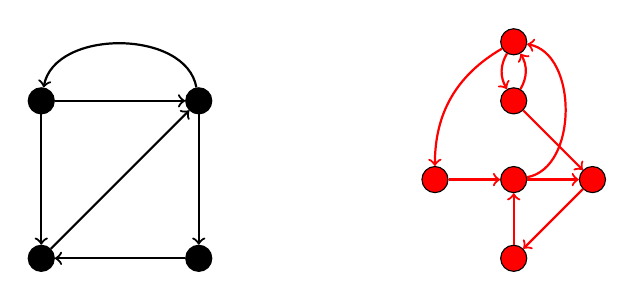
\begin{tikzpicture}[baseline=(current bounding box.north),-,auto,node distance=2cm,
                    main node/.style={circle,draw,fill=black,font=\sffamily\bfseries}]

  \node[main node] (1) {};
  \node[main node] (2) [right of=1] {};
  \node[main node] (3) [below of=1] {};
  \node[main node] (4) [below of=2] {};
  

  \path[thick,->]
  (1) edge (2);
  
  \path[thick,->,bend right=80]
  (2) edge (1);
  
  \path[thick,->]
  (2) edge (4)
  (4) edge (3)
  (1) edge (3)
  (3) edge (2);
  
  \node[main node,fill=red] (1a) [shift={(6,0)}] at (1) {};
  \node[main node,fill=red] (2a) [shift={(0,0.75)}] at (1a) {};
  \node[main node,fill=red] (3a) [shift={(1,-1)}] at (1a) {};
  \node[main node,fill=red] (4a) [shift={(0,-2)}] at (1a) {};
  \node[main node,fill=red] (5a) [shift={(-1,-1)}] at (1a) {};
  \node[main node,fill=red] (6a) [shift={(0,-1)}] at (1a) {};
  
  \path[thick,->,bend right=30,red]
  (1a) edge (2a);
  
   \path[thick,->,bend right=30,red]
  (2a) edge (1a)
  (2a) edge (5a);
  
   \path[thick,->,red]
   (1a) edge (3a)
   (3a) edge (4a)
   (4a) edge (6a)
   (5a) edge (6a)
   (6a) edge (3a);
   
   \path[thick,->,bend right=80,red]
   (6a) edge (2a); 
 
\end{tikzpicture}
\caption{A graph $G$ and its directed edge-vertex dual, $EV(G)$}
\end{myfigure}

This gives us a direction conversion between the current problem and a related problem to that which has already been solved.

Now to look at solving the normal node problem, when we have directed edges, well this restriction just restricts the action space (and therefore what we count as adjacent) so the heuristics still stand.

Hence for we have a solution for our problem, convert to the edge-vertex dual and then solve as before.

This will lead to the same index as before.

However we have a few weird points to look at
\begin{itemize}
\item Is there a problem if one node has no adjacent nodes (this would disconnect the graph and lead to a problem with our assumptions)
\end{itemize}

%End of main part of document
\bibliography{mybib}

\appendix
\pagenumbering{roman}
\appendixpage
\addappheadtotoc

\section{Theorem on Index}
\label{Appendix: theorem on index}
\begin{proof}
We will prove each statement seperately
\begin{itemize}
\item To see its non-decreasing observe that
\begin{align*}
W(m+1)-W(m)= c(m+1) \lambda \Bigg(E_{Y} \left[\int_{m+2-2Y}^{m+3-2Y} P(X \leq t) dt -\int_{m+1-2Y}^{m+2-2Y} P(X \leq t)dt \right] \Bigg) \geq 0
\end{align*}
we note that the fact that it is greater than 0 is due to the fact that $P(X \leq t )$ is a non-decreasing function.
\end{itemize}

\item To derive that $m$ is optimal for $\omega \in [W(m-1),W(m)]$ we shall show that the objective function, $f(m)$ is non-increasing for $m' \leq m$ and non-decreasing for $m' \geq m$.
Now 
$$f(m')-f(m'-1)=\frac{1}{m'(m'-1)} (W(m'-1)-\omega) \leq \frac{1}{m'(m'-1)} (W(m'-1)-W(m)) \leq 0$$
and
$$f(m'+1)-f(m')=\frac{1}{m'(m'+1)} (W(m') -\omega) \geq \frac{1}{m'(m'+1)} (W(m')-W(m)) \geq 0$$

\item Finally we note that $f(m+1) \leq f(m) \iff \omega \geq W(m)$. It is not optimal to visit at all if $f(m+1) \leq f(m) \, \forall m$, or equivalently
if $$\omega \geq W(m) \, \forall m \iff \omega \geq \sup\limits_{m=0,1,...} W(m)=\lim\limits_{m \rightarrow \infty} W(m)=c \lambda (1+ E[x-2Y])$$
\end{proof}

\end{document}
